% Options for packages loaded elsewhere
\PassOptionsToPackage{unicode}{hyperref}
\PassOptionsToPackage{hyphens}{url}
\PassOptionsToPackage{dvipsnames,svgnames,x11names}{xcolor}
%
\documentclass[
  ,man,floatsintext]{apa6}
\usepackage{amsmath,amssymb}
\usepackage{lmodern}
\usepackage{iftex}
\ifPDFTeX
  \usepackage[T1]{fontenc}
  \usepackage[utf8]{inputenc}
  \usepackage{textcomp} % provide euro and other symbols
\else % if luatex or xetex
  \usepackage{unicode-math}
  \defaultfontfeatures{Scale=MatchLowercase}
  \defaultfontfeatures[\rmfamily]{Ligatures=TeX,Scale=1}
\fi
% Use upquote if available, for straight quotes in verbatim environments
\IfFileExists{upquote.sty}{\usepackage{upquote}}{}
\IfFileExists{microtype.sty}{% use microtype if available
  \usepackage[]{microtype}
  \UseMicrotypeSet[protrusion]{basicmath} % disable protrusion for tt fonts
}{}
\makeatletter
\@ifundefined{KOMAClassName}{% if non-KOMA class
  \IfFileExists{parskip.sty}{%
    \usepackage{parskip}
  }{% else
    \setlength{\parindent}{0pt}
    \setlength{\parskip}{6pt plus 2pt minus 1pt}}
}{% if KOMA class
  \KOMAoptions{parskip=half}}
\makeatother
\usepackage{xcolor}
\IfFileExists{xurl.sty}{\usepackage{xurl}}{} % add URL line breaks if available
\IfFileExists{bookmark.sty}{\usepackage{bookmark}}{\usepackage{hyperref}}
\hypersetup{
  pdftitle={Prepare APA Journal Articles with R Markdown},
  pdfauthor={Frederik Aust1,2 \& Marius Barth1},
  pdflang={en-EN},
  pdfkeywords={APA style, R, knitr, R markdown, papaja},
  colorlinks=true,
  linkcolor={blue},
  filecolor={Maroon},
  citecolor={Blue},
  urlcolor={Blue},
  pdfcreator={LaTeX via pandoc}}
\urlstyle{same} % disable monospaced font for URLs
\usepackage{color}
\usepackage{fancyvrb}
\newcommand{\VerbBar}{|}
\newcommand{\VERB}{\Verb[commandchars=\\\{\}]}
\DefineVerbatimEnvironment{Highlighting}{Verbatim}{commandchars=\\\{\}}
% Add ',fontsize=\small' for more characters per line
\usepackage{framed}
\definecolor{shadecolor}{RGB}{248,248,248}
\newenvironment{Shaded}{\begin{snugshade}}{\end{snugshade}}
\newcommand{\AlertTok}[1]{\textcolor[rgb]{0.94,0.16,0.16}{#1}}
\newcommand{\AnnotationTok}[1]{\textcolor[rgb]{0.56,0.35,0.01}{\textbf{\textit{#1}}}}
\newcommand{\AttributeTok}[1]{\textcolor[rgb]{0.77,0.63,0.00}{#1}}
\newcommand{\BaseNTok}[1]{\textcolor[rgb]{0.00,0.00,0.81}{#1}}
\newcommand{\BuiltInTok}[1]{#1}
\newcommand{\CharTok}[1]{\textcolor[rgb]{0.31,0.60,0.02}{#1}}
\newcommand{\CommentTok}[1]{\textcolor[rgb]{0.56,0.35,0.01}{\textit{#1}}}
\newcommand{\CommentVarTok}[1]{\textcolor[rgb]{0.56,0.35,0.01}{\textbf{\textit{#1}}}}
\newcommand{\ConstantTok}[1]{\textcolor[rgb]{0.00,0.00,0.00}{#1}}
\newcommand{\ControlFlowTok}[1]{\textcolor[rgb]{0.13,0.29,0.53}{\textbf{#1}}}
\newcommand{\DataTypeTok}[1]{\textcolor[rgb]{0.13,0.29,0.53}{#1}}
\newcommand{\DecValTok}[1]{\textcolor[rgb]{0.00,0.00,0.81}{#1}}
\newcommand{\DocumentationTok}[1]{\textcolor[rgb]{0.56,0.35,0.01}{\textbf{\textit{#1}}}}
\newcommand{\ErrorTok}[1]{\textcolor[rgb]{0.64,0.00,0.00}{\textbf{#1}}}
\newcommand{\ExtensionTok}[1]{#1}
\newcommand{\FloatTok}[1]{\textcolor[rgb]{0.00,0.00,0.81}{#1}}
\newcommand{\FunctionTok}[1]{\textcolor[rgb]{0.00,0.00,0.00}{#1}}
\newcommand{\ImportTok}[1]{#1}
\newcommand{\InformationTok}[1]{\textcolor[rgb]{0.56,0.35,0.01}{\textbf{\textit{#1}}}}
\newcommand{\KeywordTok}[1]{\textcolor[rgb]{0.13,0.29,0.53}{\textbf{#1}}}
\newcommand{\NormalTok}[1]{#1}
\newcommand{\OperatorTok}[1]{\textcolor[rgb]{0.81,0.36,0.00}{\textbf{#1}}}
\newcommand{\OtherTok}[1]{\textcolor[rgb]{0.56,0.35,0.01}{#1}}
\newcommand{\PreprocessorTok}[1]{\textcolor[rgb]{0.56,0.35,0.01}{\textit{#1}}}
\newcommand{\RegionMarkerTok}[1]{#1}
\newcommand{\SpecialCharTok}[1]{\textcolor[rgb]{0.00,0.00,0.00}{#1}}
\newcommand{\SpecialStringTok}[1]{\textcolor[rgb]{0.31,0.60,0.02}{#1}}
\newcommand{\StringTok}[1]{\textcolor[rgb]{0.31,0.60,0.02}{#1}}
\newcommand{\VariableTok}[1]{\textcolor[rgb]{0.00,0.00,0.00}{#1}}
\newcommand{\VerbatimStringTok}[1]{\textcolor[rgb]{0.31,0.60,0.02}{#1}}
\newcommand{\WarningTok}[1]{\textcolor[rgb]{0.56,0.35,0.01}{\textbf{\textit{#1}}}}
\usepackage{graphicx}
\makeatletter
\def\maxwidth{\ifdim\Gin@nat@width>\linewidth\linewidth\else\Gin@nat@width\fi}
\def\maxheight{\ifdim\Gin@nat@height>\textheight\textheight\else\Gin@nat@height\fi}
\makeatother
% Scale images if necessary, so that they will not overflow the page
% margins by default, and it is still possible to overwrite the defaults
% using explicit options in \includegraphics[width, height, ...]{}
\setkeys{Gin}{width=\maxwidth,height=\maxheight,keepaspectratio}
% Set default figure placement to htbp
\makeatletter
\def\fps@figure{htbp}
\makeatother
\setlength{\emergencystretch}{3em} % prevent overfull lines
\providecommand{\tightlist}{%
  \setlength{\itemsep}{0pt}\setlength{\parskip}{0pt}}
\setcounter{secnumdepth}{-\maxdimen} % remove section numbering
% Make \paragraph and \subparagraph free-standing
\ifx\paragraph\undefined\else
  \let\oldparagraph\paragraph
  \renewcommand{\paragraph}[1]{\oldparagraph{#1}\mbox{}}
\fi
\ifx\subparagraph\undefined\else
  \let\oldsubparagraph\subparagraph
  \renewcommand{\subparagraph}[1]{\oldsubparagraph{#1}\mbox{}}
\fi
\newlength{\cslhangindent}
\setlength{\cslhangindent}{1.5em}
\newlength{\csllabelwidth}
\setlength{\csllabelwidth}{3em}
\newlength{\cslentryspacingunit} % times entry-spacing
\setlength{\cslentryspacingunit}{\parskip}
\newenvironment{CSLReferences}[2] % #1 hanging-ident, #2 entry spacing
 {% don't indent paragraphs
  \setlength{\parindent}{0pt}
  % turn on hanging indent if param 1 is 1
  \ifodd #1
  \let\oldpar\par
  \def\par{\hangindent=\cslhangindent\oldpar}
  \fi
  % set entry spacing
  \setlength{\parskip}{#2\cslentryspacingunit}
 }%
 {}
\usepackage{calc}
\newcommand{\CSLBlock}[1]{#1\hfill\break}
\newcommand{\CSLLeftMargin}[1]{\parbox[t]{\csllabelwidth}{#1}}
\newcommand{\CSLRightInline}[1]{\parbox[t]{\linewidth - \csllabelwidth}{#1}\break}
\newcommand{\CSLIndent}[1]{\hspace{\cslhangindent}#1}
\ifLuaTeX
\usepackage[bidi=basic]{babel}
\else
\usepackage[bidi=default]{babel}
\fi
\babelprovide[main,import]{english}
% get rid of language-specific shorthands (see #6817):
\let\LanguageShortHands\languageshorthands
\def\languageshorthands#1{}
% Manuscript styling
\usepackage{upgreek}
\captionsetup{font=singlespacing,justification=justified}

% Table formatting
\usepackage{longtable}
\usepackage{lscape}
% \usepackage[counterclockwise]{rotating}   % Landscape page setup for large tables
\usepackage{multirow}		% Table styling
\usepackage{tabularx}		% Control Column width
\usepackage[flushleft]{threeparttable}	% Allows for three part tables with a specified notes section
\usepackage{threeparttablex}            % Lets threeparttable work with longtable

% Create new environments so endfloat can handle them
% \newenvironment{ltable}
%   {\begin{landscape}\centering\begin{threeparttable}}
%   {\end{threeparttable}\end{landscape}}
\newenvironment{lltable}{\begin{landscape}\centering\begin{ThreePartTable}}{\end{ThreePartTable}\end{landscape}}

% Enables adjusting longtable caption width to table width
% Solution found at http://golatex.de/longtable-mit-caption-so-breit-wie-die-tabelle-t15767.html
\makeatletter
\newcommand\LastLTentrywidth{1em}
\newlength\longtablewidth
\setlength{\longtablewidth}{1in}
\newcommand{\getlongtablewidth}{\begingroup \ifcsname LT@\roman{LT@tables}\endcsname \global\longtablewidth=0pt \renewcommand{\LT@entry}[2]{\global\advance\longtablewidth by ##2\relax\gdef\LastLTentrywidth{##2}}\@nameuse{LT@\roman{LT@tables}} \fi \endgroup}

% \setlength{\parindent}{0.5in}
% \setlength{\parskip}{0pt plus 0pt minus 0pt}

% Overwrite redefinition of paragraph and subparagraph by the default LaTeX template
% See https://github.com/crsh/papaja/issues/292
\makeatletter
\renewcommand{\paragraph}{\@startsection{paragraph}{4}{\parindent}%
  {0\baselineskip \@plus 0.2ex \@minus 0.2ex}%
  {-1em}%
  {\normalfont\normalsize\bfseries\itshape\typesectitle}}

\renewcommand{\subparagraph}[1]{\@startsection{subparagraph}{5}{1em}%
  {0\baselineskip \@plus 0.2ex \@minus 0.2ex}%
  {-\z@\relax}%
  {\normalfont\normalsize\itshape\hspace{\parindent}{#1}\textit{\addperi}}{\relax}}
\makeatother

% \usepackage{etoolbox}
\makeatletter
\patchcmd{\HyOrg@maketitle}
  {\section{\normalfont\normalsize\abstractname}}
  {\section*{\normalfont\normalsize\abstractname}}
  {}{\typeout{Failed to patch abstract.}}
\patchcmd{\HyOrg@maketitle}
  {\section{\protect\normalfont{\@title}}}
  {\section*{\protect\normalfont{\@title}}}
  {}{\typeout{Failed to patch title.}}
\makeatother

\usepackage{xpatch}
\makeatletter
\xapptocmd\appendix
  {\xapptocmd\section
    {\addcontentsline{toc}{section}{\appendixname\ifoneappendix\else~\theappendix\fi\\: #1}}
    {}{\InnerPatchFailed}%
  }
{}{\PatchFailed}
\keywords{APA style, R, knitr, R markdown, papaja\newline\indent Word count: ~3147}
\usepackage{lineno}

\linenumbers
\usepackage{csquotes}
\usepackage{fvextra}
\usepackage{csquotes}
\usepackage{subfig}
\renewcommand*{\thesubfigure}{\MakeUppercase{\alph{subfigure}}}
\raggedbottom
\ifLuaTeX
  \usepackage{selnolig}  % disable illegal ligatures
\fi

\title{Prepare APA Journal Articles with R Markdown}
\author{Frederik Aust\textsuperscript{1,2} \& Marius Barth\textsuperscript{1}}
\date{}


\shorttitle{\textbf{papaja}}

\authornote{

The authors made the following contributions. Frederik Aust: Conceptualization, Writing---Original Draft Preparation, Writing---Review \& Editing, Software, Project administration; Marius Barth: Conceptualization, Writing---Review \& Editing, Software.

Correspondence concerning this article should be addressed to Frederik Aust, Department Psychology, University of Cologne, Herbert-Lewin-Str. 2, 50931 Köln, Germany. E-mail: \href{mailto:frederik.aust@uni-koeln.de}{\nolinkurl{frederik.aust@uni-koeln.de}}

}

\affiliation{\vspace{0.5cm}\textsuperscript{1} University of Cologne\\\textsuperscript{2} University of Amsterdam}

\abstract{%
\textbf{papaja} addresses computational non-reproducibility in research reports caused by reporting errors, i.e.~incomplete or incorrect reporting of the analytic procedure or analytic results. The package is tailored to authors of scientific manuscripts that must adhere to the guidelines of the American Psychological Society (6th edition). This document was written with \textbf{papaja} and provides a brief overview of the package's main features: An R Markdown template for APA-style manuscripts and helper-functions that facilitate reporting of analytic results in accordance with APA guidelines.
}



\begin{document}
\maketitle



Computational reproducibility is of fundamental importance to the quantitative sciences (Cacioppo, Kaplan, Krosnick, Olds, \& Dean, 2015; Donoho, 2010; Hutson, 2018; Peng, 2011).
Yet, non-reproducible results are widely prevalent.
Computational reproducibility is threatened by countless sources of errors, but among the most common problems are incomplete or incorrect reporting of statistical procedures and results (Artner et al., 2020).
\textbf{papaja} was designed to address these problems.
The package is tailored to authors of scientific manuscripts that must adhere to the guidelines of the American Psychological Association (APA, 6th edition, American Psychological Association, 2010).
\textbf{papaja} provides \href{https://rmarkdown.rstudio.com/}{\textbf{rmarkdown}} (Xie, Allaire, \& Grolemund, 2018) templates to create DOCX documents and PDF documents---using \LaTeX document class \href{http://www.ctan.org/pkg/apa6}{\texttt{apa6}}.
Moreover, \textbf{papaja} provides helper functions to facilitate the reporting of results of your analyses in accordance with APA guidelines.
This document was written with \textbf{papaja} and provides a brief overview of the package's main features.
For a comprehensive introduction and installation instructions, see the current draft of the \href{http://frederikaust.com/papaja_man/}{\textbf{papaja} manual}.\footnote{If you have a specific question that is not answered in the manual, feel free to ask a question on Stack Overflow using the \href{https://stackoverflow.com/questions/tagged/papaja}{\textbf{papaja} tag}.
  If you believe you have found a bug or would like to request a new feature, \href{https://github.com/crsh/papaja/issues}{open an issue} on Github and provide a \href{https://stackoverflow.com/help/mcve}{minimal complete verifiable example}.}

\hypertarget{the-problem-copy-paste-reporting}{%
\section{The problem: Copy-paste reporting}\label{the-problem-copy-paste-reporting}}

Readers of scientific journal articles generally assume that numerical results and figures directly flow from the underlying data and analytic procedure.
Execution of analyses and reporting of results are typically not considered sources of error that threaten the validity of scientific claims---the computational reproducibility of the reported results is a forgone conclusion.
The natural assumption of computational reproducibility reflects its fundamental importance to quantitative sciences as acknowledged by the U.S.
National Science Foundation subcommittee on Replicability in Science:

\begin{quote}
{[}Computational{]} Reproducibility is a minimum necessary condition for a finding to be believable and informative.
(p.~4, Cacioppo et al., 2015)
\end{quote}

Non-reproducible results are scientifically and ethically unacceptable.
They impede an accumulation of knowledge, waste resources, and when applied could have serious consequences.
A recent investigation of breast cancer treatments erroneously concluded that radiotherapy after mastectomy increased mortality because of an error in the analysis code (Henson et al., 2016).
A corrected reanalysis indicated that, in fact, the opposite was the case---the treatment appeared to be effectively decrease mortality.
Examples like this show that computational reproducibility cannot be a forgone conclusion.

Large-scale scrutiny of statistics published in over 30,000 articles in psychology journals shows that every other article reports at least one impossible combination of test statistic, degrees of freedom, and \(p\) value; in every tenth article such inconsistencies call the statistical inference into question (Nuijten, Hartgerink, Assen, Epskamp, \& Wicherts, 2016).
More in-depth investigations that attempted to reproduce reported results from the underlying raw data paint a similar picture.
For example, in a sample of 46 articles, two thirds of key claims could be reproduced but in every tenth case only after deviating from the reported analysis plan (Artner et al., 2020).
For one in four non-reproducible results, the reproduction attempt yielded results that were no longer statistically significant, calling the original statistical inference into question.
These figures clearly show that there is a need for efforts to improve the computational reproducibility of the published literature.

Computational non-reproducibility is, of course, multi-causal.
While there is only one way in which a research report is computationally reproducible, the is a countless number of things that can go wrong.
Broadly speaking, there are at least four causes for non-reproducible analyses: (1) incomplete or incorrect reporting of the analytic procedure, (2) incorrect execution of the analytic procedure, (3) incorrect reporting of results, and (4) code rot, i.e., non-reproducible caused by (inadvertent) changes to the computational environment (e.g., software updates, changes to data files).
We currently see no technical solution to the first two causes.
Incomplete reporting (1) may be partially mitigated by strictly enforcing reporting guidelines.
However, verifying that the analytic procedure is reported faithfully (1) and was executed correctly (2) ultimately requires manual scrutiny of analysis scripts and/or reproduction and is possible only if authors share their data.
Code rot (4), on the other hand, can be adequately addressed by conserving the software environment in which the results were produced (e.g., R and all R packages).
Several seasoned technical solutions, such as software containers or a virtual machine, exist (Grüning et al., 2018; Piccolo \& Frampton, 2016).\footnote{\textbf{papaja} can be readily combined with these tools as documented in the section on \href{http://frederikaust.com/papaja_man/tips-and-tricks.html\#reproducible-software-environments}{reproducible software environments} in the \textbf{papaja} manual.}
\textbf{papaja} provides a technical safeguard for correct reporting of results (3).

When it comes to reporting quantitative results, most researchers engage in what we refer to as \emph{copy-paste reporting}.
Quantitative analyses and reporting are done in separate software.
Thus, by necessity quantitative results are copied from the analysis software and pasted into the report.
Copy-paste reporting underlies and contributes to several of the most common causes for computational non-reproducibility: Rounding errors, incorrect labeling of statistical results, typos, and inserting results of a different analysis (pp.~12-13, Artner et al., 2020).
We are convinced that errors caused by copy-paste reporting cannot be addressed by appealing to researchers to be more careful.
The motivation to avoid such errors should already be high because the reputational cost of errata and retractions due to non-reproducible results is substantial.
Even researchers that open their data (and analysis code) to the public or anticipate systematic editorial scrutiny report non-reproducible results (Eubank, 2016; Hardwicke et al., 2018; Obels, Lakens, Coles, Gottfried, \& Green, 2020).
Evidently, computational reproducibility is difficult to attain.

\hypertarget{the-solution-dynamic-documents}{%
\section{The solution: Dynamic documents}\label{the-solution-dynamic-documents}}

We believe copy-paste reporting is a flawed approach to reporting quantitative results.
Hence, we believe researchers need stop copy-pasting to safeguard the computational reproducibility of their manuscripts.
Manuscripts should be dynamic (or \enquote{living}) documents (Knuth, 1984; Xie et al., 2018) that contain direct links to the analytic software.
Dynamic documents fuse analysis code and prose such that statistics, figures, and tables are automatically inserted into a manuscript---and updated as data or analysis code change.
As an added benefit, dynamic documents have great potential to improve the computational reproducibility of manuscripts beyond reporting errors as they facilitate independent reproduction.
Dynamic documents fully document the analytic procedure and establish direct links to the associated scientific claims.

\textbf{papaja}, and \href{http://frederikaust.com/papaja_man/introduction.html\#document-compilation}{the software it builds on}, provides researchers with the tools to create dynamic submission-ready manuscripts in the widely used APA style.
The dominant approach to creating dynamic documents in R is to use the \href{https://rmarkdown.rstudio.com/}{\textbf{rmarkdown}} package (Xie et al., 2018).
\textbf{papaja} provides R Markdown templates to create DOCX and PDF documents (using \LaTeX document class \texttt{apa6}).
Moreover, \textbf{papaja} provides several functions to conveniently report analytic results according to APA guidelines.
The remainder of this document illustrates how these functions can be used.

\hypertarget{setting-up-a-new-document}{%
\section{Setting up a new document}\label{setting-up-a-new-document}}

Once \textbf{papaja} and all other \href{http://frederikaust.com/papaja_man/introduction.html\#software-requirements}{required software} is installed, the APA template is available through the RStudio menu, see Figure~\ref{fig:rstudio}.
When you click RStudio's \emph{Knit} button, a manuscript conforming to APA style is rendered, which includes both your text and the output of any embedded R code chunks within the manuscript.
Of course, a new document can also be created without RStudio using \texttt{rmarkdown::draft()} and rendered using \texttt{rmarkdown::render()}.

\begin{Shaded}
\begin{Highlighting}[]
\CommentTok{\# Create new R Markdown file}
\NormalTok{rmarkdown}\SpecialCharTok{::}\FunctionTok{draft}\NormalTok{(}
  \StringTok{"manuscript.Rmd"}
\NormalTok{  , }\StringTok{"apa6"}
\NormalTok{  , }\AttributeTok{package =} \StringTok{"papaja"}
\NormalTok{  , }\AttributeTok{create\_dir =} \ConstantTok{FALSE}
\NormalTok{  , }\AttributeTok{edit =} \ConstantTok{FALSE}
\NormalTok{)}

\CommentTok{\# Render manuscript}
\NormalTok{rmarkdown}\SpecialCharTok{::}\FunctionTok{render}\NormalTok{(}\StringTok{"manuscript.Rmd"}\NormalTok{)}
\end{Highlighting}
\end{Shaded}



\begin{figure}

{\centering 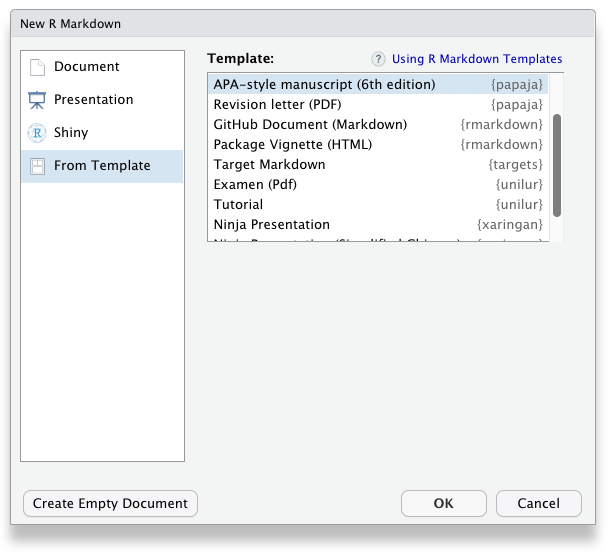
\includegraphics[width=3.9in]{../inst/images/template_selection} 

}

\caption{After successful installation the \textbf{papaja} APA manuscript template is available via the RStudio menu.}\label{fig:rstudio}
\end{figure}

This document is in APA manuscript style, but other styles are available for PDF documents.
The document style can be controlled via the \texttt{classoption} field of the YAML front matter.
For a thesis-like style change \texttt{classoption} to \texttt{doc} or use \texttt{jou} for a more polished journal-like two-column layout.
For a comprehensive overview of other formatting options please refer to the \href{http://frederikaust.com/papaja_man/r-markdown-components.html\#rendering-options}{\textbf{papaja} manual}.

To create DOCX documents, the \texttt{output} field in the YAML front matter can be set to \texttt{papaja::apa6\_docx}.
Please note, however, that DOCX documents are somewhat less flexible and less polished than PDF documents.
\textbf{papaja} builds on \texttt{pandoc} to render Markdown into PDF and DOCX documents.
Unfortunately, \texttt{pandoc}'s capabilities are more limited for DOCX documents.
This is why some \textbf{papaja} features are only available for PDF documents, for example, see the summary of \href{http://frederikaust.com/papaja_man/r-markdown-components.html\#rendering-options}{rendering options} in the manual.
Also, DOCX documents require some \href{http://frederikaust.com/papaja_man/limitations.html\#microsoft-word-documents}{limited manual work} before they fully comply with APA guidelines.
The DOCX documents produced by \textbf{papaja} should, however, be suitable for collaboration with colleagues, who prefer Word over R Markdown and to prepare journal submissions.

\hypertarget{writing}{%
\section{Writing}\label{writing}}

Like \textbf{rmarkdown}, \textbf{papaja} uses Markdown syntax to format text.
A comprehensive overview of the supported Markdown syntax is available in the \href{https://pandoc.org/MANUAL.html\#pandocs-markdown}{\texttt{pandoc} manual}.
In the following, we will highlight a few features that are of particular relevance to the technical writing of research reports.

\hypertarget{citations}{%
\subsection{Citations}\label{citations}}

By default, citations in \textbf{papaja} are processed by the \texttt{pandoc} extension \texttt{citeproc}, which works well for both PDF and DOCX documents.
\texttt{citeproc} takes reference information from a bibliography file, which can be in one of several formats (e.g., CSL-JSON, Bib(La)TeX, EndNote, RIS, Medline).
To start citing, specify the path to the bibliography file in \texttt{bibliography} field of the YAML front matter.
Once \texttt{citeproc} knows where to look for reference information, \texttt{{[}@james\_1890{]}} will render to a citation within parentheses, i.e., (James, 1890).
Multiple citations must be separated by a semicolon \texttt{;} (e.g., \texttt{{[}@james\_1890;\ @bem\_2011{]}}) and are automatically ordered alphabetically as per APA style, i.e., (Bem, 2011; James, 1890).
To cite a source in text simply omit the brackets.
The \texttt{pandoc} manual provides a comprehensive overview of \href{https://pandoc.org/MANUAL.html\#citations}{\texttt{citeproc}} and the supported \href{https://pandoc.org/MANUAL.html\#citation-syntax}{citation syntax}.

To facilitate inserting citations, you may use the RStudio Visual Editor's \href{https://rstudio.github.io/visual-markdown-editing/citations.html\#inserting-citations}{bibliography search} and auto-completion of reference handles.
If you use VSCode with the \href{https://marketplace.visualstudio.com/items?itemName=Ikuyadeu.r}{R extension} or RStudio without the Visual Editor, the add-in provided in \href{https://github.com/crsh/citr}{\textbf{citr}} serves a similar purpose.
Both the Visual Editor and \textbf{citr} can also access your Zotero database directly and copy references to your bibliography file.

As academics and open source developers, we believe it is important to credit the software we use for our publications.
A lot of R packages are developed by academics free of charge.
As citations are the currency of academia, it is easy to compensate volunteers for their work by citing their R packages.
\textbf{papaja} provides two functions that make citing R and its packages quite convenient:

\texttt{r\_refs()} creates a BibLaTeX file containing citations for R and all currently loaded packages.
\texttt{cite\_r()} takes these citations and turns them into readily reportable text.
\texttt{my\_citation} now contains the following text that you can use in your document:

\begin{Verbatim}[breaklines=true]
R [Version 4.1.2\; @R-base] and the R-packages *afex* [Version 1.0.1\; @R-afex], *dplyr* [Version 1.0.8\; @R-dplyr], *ggforce* [Version 0.3.3\; @R-ggforce], *ggplot2* [Version 3.3.5\; @R-ggplot2], *lme4* [Version 1.1.28\; @R-lme4], *Matrix* [Version 1.3.4\; @R-Matrix], *papaja* [Version 0.2.0\; @R-papaja], and *tinylabels* [Version 0.2.3\; @R-tinylabels]
\end{Verbatim}

\hypertarget{equations}{%
\subsection{Equations}\label{equations}}

Equations can be reported using the powerful \LaTeX syntax.
Inline math must be enclosed in \texttt{\$} or \texttt{\textbackslash{}(} and \texttt{\textbackslash{})}, for example, \texttt{\$d\textquotesingle{}\ =\ z(H)\ -\ z(\textbackslash{}mathit\{FA\})\$}, which renders to \(d' = z(H) - z(\mathit{FA})\).
For larger formulas, displayed equations are more appropriate; they are enclosed in \texttt{\$\$} or \texttt{\textbackslash{}{[}}and \texttt{\textbackslash{}{]}}, and will, for example, render to

\[
d' = \frac{\mu_{old} - \mu_{new}}{\sqrt{0.5(\sigma^2_{old} + \sigma^2_{new})}}.
\]

\hypertarget{reporting-results}{%
\section{Reporting results}\label{reporting-results}}

If you are not familiar with R Markdown and how it can be used to conduct and document your analyses, we recommend you familiarize yourself with R Markdown first.
RStudio provides a \href{https://rmarkdown.rstudio.com/lesson-1.html}{concise introduction}.

\texttt{apa\_print()} is a core function in \textbf{papaja} to facilitate reporting analytic results for a growing number of analytic output objects, Table~\ref{tab:apa-print-methods}.
Consider the following example of an analysis of variance.
After performing the analysis, the result is passed to \texttt{apa\_print()}.
The function takes the R object returned by the analysis function and returns a list that contains reportable text and tables.

\begin{Shaded}
\begin{Highlighting}[]
\NormalTok{recall\_anova }\OtherTok{\textless{}{-}}\NormalTok{ afex}\SpecialCharTok{::}\FunctionTok{aov\_4}\NormalTok{(}
\NormalTok{  Recall }\SpecialCharTok{\textasciitilde{}}\NormalTok{ (Task }\SpecialCharTok{*}\NormalTok{ Valence }\SpecialCharTok{*}\NormalTok{ Dosage) }\SpecialCharTok{+}\NormalTok{ (Task }\SpecialCharTok{*}\NormalTok{ Valence }\SpecialCharTok{|}\NormalTok{ Subject)}
\NormalTok{  , }\AttributeTok{data =}\NormalTok{ mixed\_data}
\NormalTok{)}
\NormalTok{recall\_anova\_results }\OtherTok{\textless{}{-}} \FunctionTok{apa\_print}\NormalTok{(recall\_anova)}
\FunctionTok{str}\NormalTok{(recall\_anova\_results)}
\end{Highlighting}
\end{Shaded}

\begin{footnotesize}

\begin{verbatim}
## List of 4
## $ estimate :List of 7
## ..$ Dosage : chr "$\\hat{\\eta}^2_G = .267$, 90\\% CI $[.000, .507]$"
## ..$ Task : chr "$\\hat{\\eta}^2_G = .048$, 90\\% CI $[.000, .297]$"
## ..$ Valence : chr "$\\hat{\\eta}^2_G = .008$, 90\\% CI $[.000, .052]$"
## .. [list output truncated]
## $ statistic :List of 7
## ..$ Dosage : chr "$F(2, 15) = 2.97$, $p = .082$"
## ..$ Task : chr "$F(1, 15) = 43.13$, $p < .001$"
## ..$ Valence : chr "$F(1.62, 24.36) = 3.46$, $p = .056$"
## .. [list output truncated]
## $ full_result:List of 7
## ..$ Dosage : chr "$F(2, 15) = 2.97$, $p = .082$, $\\hat{\\eta}^2_G = .267$, 90\\% CI
##       $[.000, .507]$"
## ..$ Task : chr "$F(1, 15) = 43.13$, $p < .001$, $\\hat{\\eta}^2_G = .048$, 90\\% CI
##       $[.000, .297]$"
## ..$ Valence : chr "$F(1.62, 24.36) = 3.46$, $p = .056$, $\\hat{\\eta}^2_G = .008$,
##       90\\% CI $[.000, .052]$"
## .. [list output truncated]
## [list output truncated]
## - attr(*, "class")= chr [1:2] "apa_results" "list"
\end{verbatim}

\end{footnotesize}

The text returned by \texttt{apa\_print()} can be inserted into manuscript as usual using inline code chunks:

\begin{Shaded}
\begin{Highlighting}[]
\NormalTok{Item }\FunctionTok{valence}\NormalTok{ (}\StringTok{\textasciigrave{}}\AttributeTok{r in\_paren(recall\_anova\_results$full\_result$Valence)}\StringTok{\textasciigrave{}}\NormalTok{) and}
\NormalTok{the task affected recall performance,}
\StringTok{\textasciigrave{}}\AttributeTok{r recall\_anova\_results$full\_result$Task}\StringTok{\textasciigrave{}}\NormalTok{; the dosage, however, had no}
\NormalTok{detectable effect on recall, }\StringTok{\textasciigrave{}}\AttributeTok{r recall\_anova\_results$full\_result$Dosage}\StringTok{\textasciigrave{}}\NormalTok{.}
\NormalTok{There was no detectable interaction.}
\end{Highlighting}
\end{Shaded}

The above excerpt from an R Markdown document yields the following in the rendered document.
Note that the function \texttt{in\_paren()} replaces parentheses with brackets as per APA guidelines when statistics are reported in parentheses.

\begin{quote}
Item valence (\(F[1.62, 24.36] = 3.46\), \(p = .056\), \(\hat{\eta}^2_G = .008\), 90\% CI \([.000, .052]\)) and the task affected recall performance, \(F(1, 15) = 43.13\), \(p < .001\), \(\hat{\eta}^2_G = .048\), 90\% CI \([.000, .297]\); the dosage, however, had no effect on recall, \(F(2, 15) = 2.97\), \(p = .082\), \(\hat{\eta}^2_G = .267\), 90\% CI \([.000, .507]\).
There was no significant interaction.
\end{quote}



\begin{table}[tbp]

\begin{center}
\begin{threeparttable}

\caption{\label{tab:apa-print-methods}Object classes currently supported by \texttt{apa\_print()}.}

\begin{tabular}{llll}
\toprule
A-B & \multicolumn{1}{c}{D-L} & \multicolumn{1}{c}{L-S} & \multicolumn{1}{c}{S-Z}\\
\midrule
afex\_aov & default & lsmobj & summary.aovlist\\
anova & emmGrid & manova & summary.glht*\\
anova.lme & glht* & merMod & summary.glm\\
Anova.mlm & glm & mixed & summary.lm\\
aov & htest & papaja\_wsci & summary.manova\\
aovlist & list & summary\_emm & summary.ref.grid\\
BFBayesFactor* & lm & summary.Anova.mlm & \\
BFBayesFactorTop* & lme & summary.aov & \\
\bottomrule
\addlinespace
\end{tabular}

\begin{tablenotes}[para]
\normalsize{\textit{Note.} * These methods are not fully tested; don't trust blindly!}
\end{tablenotes}

\end{threeparttable}
\end{center}

\end{table}

In addition to individual text strings, \texttt{apa\_print()} also summarizes all results in a standardized \texttt{data.frame}.\footnote{For more complex analyses the \texttt{table} element may contain a named list of multiple tables.}
The column names conform to the \href{https://www.tidymodels.org/learn/develop/broom/\#glossary}{naming conventions} used in the \textbf{broom} package (e.g.~\texttt{estimate}, \texttt{statistic}, and \texttt{p.value}).
\texttt{apa\_print()} assigns each column an additional descriptive variable label.

\begin{Shaded}
\begin{Highlighting}[]
\FunctionTok{head}\NormalTok{(recall\_anova\_results}\SpecialCharTok{$}\NormalTok{table, }\DecValTok{3}\NormalTok{)}
\end{Highlighting}
\end{Shaded}

\begin{verbatim}
## A data.frame with 7 labelled columns:
## 
##      term estimate     conf.int statistic   df df.residual p.value
## 1  Dosage     .267 [.000, .507]      2.97    2          15    .082
## 2    Task     .048 [.000, .297]     43.13    1          15  < .001
## 3 Valence     .008 [.000, .052]      3.46 1.62       24.36    .056
## 
## term     : Effect 
## estimate : $\\hat{\\eta}^2_G$ 
## conf.int : 90\\% CI 
## statistic: $F$ 
## df       : $\\mathit{df}^{\\mathrm{GG}}$ 
## ... (2 more labels)
\end{verbatim}

\hypertarget{tables}{%
\subsection{Tables}\label{tables}}

Tables returned by \texttt{apa\_print()} can be conveniently included in a manuscript by passing them to \texttt{apa\_table()}.
This function was designed with exemplary tables from the APA manual in mind and to work well with \texttt{apa\_print()}.
Conveniently, \texttt{apa\_table()} uses any available variable labels as informative column headers, Table~\ref{tab:anova-table}.
Unfortunately, table formatting is somewhat limited for DOCX documents due to the limited table representation in \texttt{pandoc} (e.g., it is currently not possible span header cells across multiple columns or have multiple header rows).
Of course, popular packages for creating tables, such as \href{https://haozhu233.github.io/kableExtra/}{\textbf{kableExtra}}, \href{https://hughjonesd.github.io/huxtable/}{\textbf{huxtable}}, or \href{https://ardata-fr.github.io/flextable-book/index.html}{\textbf{flextable}} can also be used and may be preferable for more complex tables.





\begin{table}[tbp]

\begin{center}
\begin{threeparttable}

\caption{\label{tab:anova-table}ANOVA table for recall performance as a function of task, valence, and dosage.}

\begin{tabular}{lrcrllr}
\toprule
Effect & \multicolumn{1}{c}{$\hat{\eta}^2_G$} & \multicolumn{1}{c}{90\% CI} & \multicolumn{1}{c}{$F$} & \multicolumn{1}{c}{$\mathit{df}^{\mathrm{GG}}$} & \multicolumn{1}{c}{$\mathit{df}_{\mathrm{res}}^{\mathrm{GG}}$} & \multicolumn{1}{c}{$p$}\\
\midrule
Dosage & .267 & {}[.000, .507] & 2.97 & 2 & 15 & .082\\
Task & .048 & {}[.000, .297] & 43.13 & 1 & 15 & < .001\\
Valence & .008 & {}[.000, .052] & 3.46 & 1.62 & 24.36 & .056\\ \midrule
Dosage $\times$ Task & .004 & {}[.000, .000] & 1.83 & 2 & 15 & .195\\
Dosage $\times$ Valence & .011 & {}[.000, .000] & 2.38 & 3.25 & 24.36 & .090\\
Task $\times$ Valence & .003 & {}[.000, .000] & 1.50 & 1.35 & 20.20 & .242\\ \midrule
Dosage $\times$ Task $\times$ Valence & .001 & {}[.000, .000] & 0.39 & 2.69 & 20.20 & .743\\
\bottomrule
\addlinespace
\end{tabular}

\begin{tablenotes}[para]
\normalsize{\textit{Note.} This is a table created using \texttt{apa\_print()} and \texttt{apa\_table()}.}
\end{tablenotes}

\end{threeparttable}
\end{center}

\end{table}

\begin{Shaded}
\begin{Highlighting}[]
\FunctionTok{apa\_table}\NormalTok{(}
\NormalTok{  recall\_anova\_results}\SpecialCharTok{$}\NormalTok{table}
\NormalTok{  , }\AttributeTok{caption =} \StringTok{"ANOVA table for recall performance as a function of task,}
\StringTok{    valence, and dosage."}
\NormalTok{  , }\AttributeTok{note =} \StringTok{"This is a table created using apa\_print() and apa\_table()."}
\NormalTok{  , }\AttributeTok{align =} \StringTok{"lrcrllr"}
\NormalTok{  , }\AttributeTok{midrules =} \FunctionTok{c}\NormalTok{(}\DecValTok{3}\NormalTok{, }\DecValTok{6}\NormalTok{)}
\NormalTok{)}
\end{Highlighting}
\end{Shaded}

As required by the APA guidelines, tables are deferred to the final pages of the manuscript when creating PDF documents.\footnote{Again, this is currently not the case in DOCX documents.}
To place tables and figures in text instead, the \texttt{floatsintext} field in the YAML header can be set to \texttt{yes}.

\hypertarget{figures}{%
\subsection{Figures}\label{figures}}

Figures generated in R are automatically inserted into the document.
\textbf{papaja} provides a set of functions built around \texttt{apa\_factorial\_plot()} that facilitate visualizing data from factorial study designs, Figure~\ref{fig:beeplots}(A).
For \textbf{ggplot2} users, \textbf{papaja} provides \texttt{theme\_apa()}, a theme designed with APA manuscript guidelines in mind, Figure~\ref{fig:beeplots}(B).

\begin{Shaded}
\begin{Highlighting}[]
\FunctionTok{apa\_beeplot}\NormalTok{(}
\NormalTok{  mixed\_data}
\NormalTok{  , }\AttributeTok{id =} \StringTok{"Subject"}
\NormalTok{  , }\AttributeTok{dv =} \StringTok{"Recall"}
\NormalTok{  , }\AttributeTok{factors =} \FunctionTok{c}\NormalTok{(}\StringTok{"Valence"}\NormalTok{, }\StringTok{"Dosage"}\NormalTok{, }\StringTok{"Task"}\NormalTok{) }
\NormalTok{  , }\AttributeTok{ylim =} \FunctionTok{c}\NormalTok{(}\DecValTok{0}\NormalTok{, }\DecValTok{30}\NormalTok{)}
\NormalTok{  , }\AttributeTok{las =} \DecValTok{1}
\NormalTok{  , }\AttributeTok{args\_points =} \FunctionTok{list}\NormalTok{(}\AttributeTok{cex =} \FloatTok{1.25}\NormalTok{)}
\NormalTok{  , }\AttributeTok{args\_arrows =} \FunctionTok{list}\NormalTok{(}\AttributeTok{length =} \FloatTok{0.025}\NormalTok{)}
\NormalTok{  , }\AttributeTok{args\_legend =} \FunctionTok{list}\NormalTok{(}\AttributeTok{x =} \StringTok{"top"}\NormalTok{, }\AttributeTok{horiz =} \ConstantTok{TRUE}\NormalTok{)}
\NormalTok{)}
\end{Highlighting}
\end{Shaded}







\begin{figure}

{\centering \subfloat[\centering Figure created using \texttt{apa\_factorial\_plot()}.\label{fig:beeplots-1}]{\includegraphics{papaja_files/figure-latex/beeplots-1} }\newline\subfloat[\centering Figure created using \texttt{ggplot()} and \texttt{theme\_apa()}.\label{fig:beeplots-2}]{\includegraphics{papaja_files/figure-latex/beeplots-2} }

}

\caption{Bee plots of the example data set. Small points represent individual observations, large points represent means, and error bars represent 95\% confidence intervals.}\label{fig:beeplots}
\end{figure}

Again, as required by the APA guidelines, figures are deferred to the final pages of the document unless the \texttt{floatsintext} field in the YAML header can be set to \texttt{yes}.

\hypertarget{referencing-tables-and-figures}{%
\subsection{Referencing tables and figures}\label{referencing-tables-and-figures}}

\textbf{papaja} builds on the \textbf{bookdown} package, which provides limited cross-referencing capabilities within documents.
By default, automatically generated table and figure numbers can be inserted into the text using \texttt{\textbackslash{}@ref(tab:chunk-name)} for tables or \texttt{\textbackslash{}@ref(fig:chunk-name)} for figures.
Note that for this syntax to work chunk names cannot include underscores (i.e., \texttt{\_}).

\hypertarget{getting-help}{%
\section{Getting help}\label{getting-help}}

For a comprehensive introduction to \textbf{papaja}, check out the current draft of the \href{http://frederikaust.com/papaja_man/}{\textbf{papaja} manual}.
If you have a specific question that is not answered in the manual, feel free to ask a question on Stack Overflow \href{https://stackoverflow.com/questions/tagged/papaja}{using the \textbf{papaja} tag}.
If you believe you have found a bug or you want to request a new feature, \href{https://github.com/crsh/papaja/issues}{open an issue} on Github and provide a \href{https://stackoverflow.com/help/mcve}{minimal complete verifiable example}.

If you are interested to see how others use \textbf{papaja}, take a look at some of the publicly available R Markdown files.
The file used to create this document is available at the \href{https://github.com/crsh/papaja/blob/master/vignettes/papaja.Rmd}{\textbf{papaja} GitHub repository}.
Moreover, a \href{http://frederikaust.com/papaja_man/published-manuscripts.html}{collection of papers} written with \textbf{papaja,} including the corresponding R Markdown files, is listed in the manual.
If you have published a paper that was written with \textbf{papaja}, please add the reference to the \href{https://www.zotero.org/groups/2202906/papaja}{public Zotero group} yourself or send us to me.

\hypertarget{contributing}{%
\section{Contributing}\label{contributing}}

If you like \textbf{papaja} and would like to contribute, we highly appreciate any contributions to the R package or its documentation.
Take a look at the \href{https://github.com/crsh/papaja/issues}{open issues} if you need inspiration.
There are many additional analyses that we would like \texttt{apa\_print()} to support; new S3/S4-methods are always appreciated (e.g., for \texttt{factanal}, \texttt{fa}, \texttt{lavaan}).
For a primer on adding new \texttt{apa\_print()}-methods, see the getting-started-vignette (\texttt{vignette("extending\_apa\_print",\ package\ =\ "papaja")}).
Before working on a contribution, please review our brief \href{https://github.com/crsh/papaja/blob/master/.github/CONTRIBUTING.md}{contributing guidelines} and \href{https://github.com/crsh/papaja/blob/master/CODE_OF_CONDUCT.md}{code of conduct}.

Enjoy writing.
:)

\pagebreak

\hypertarget{references}{%
\section{References}\label{references}}

\setlength{\parindent}{-0.5in}
\setlength{\leftskip}{0.5in}

\hypertarget{refs}{}
\begin{CSLReferences}{1}{0}
\leavevmode\vadjust pre{\hypertarget{ref-american_psychological_association_publication_2010}{}}%
American Psychological Association. (2010). \emph{Publication Manual of the American Psychological Association} (6th edition). Washington, DC: American Psychological Association.

\leavevmode\vadjust pre{\hypertarget{ref-artner_reproducibility_2020}{}}%
Artner, R., Verliefde, T., Steegen, S., Gomes, S., Traets, F., Tuerlinckx, F., \& Vanpaemel, W. (2020). The reproducibility of statistical results in psychological research: An investigation using unpublished raw data. \emph{Psychological Methods}. (2020-84997-001). \url{https://doi.org/10.1037/met0000365}

\leavevmode\vadjust pre{\hypertarget{ref-cacioppo_social_2015}{}}%
Cacioppo, J. T., Kaplan, R. M., Krosnick, J. A., Olds, J. L., \& Dean, H. (2015). \emph{Social, Behavioral, and Economic Sciences Perspectives on Robust and Reliable Science} {[}Report of the Subcommittee on Replicability in Science{]}. Arlington, VA: National Science Foundation. Retrieved from National Science Foundation website: \url{http://web.stanford.edu/group/bps/cgi-bin/wordpress/wp-content/uploads/2015/09/NSF-Robust-Research-Workshop-Report.pdf}

\leavevmode\vadjust pre{\hypertarget{ref-donoho_invitation_2010}{}}%
Donoho, D. L. (2010). An invitation to reproducible computational research. \emph{Biostatistics}, \emph{11}(3), 385--388. \url{https://doi.org/10.1093/biostatistics/kxq028}

\leavevmode\vadjust pre{\hypertarget{ref-eubank_lessons_2016}{}}%
Eubank, N. (2016). Lessons from a Decade of Replications at the Quarterly Journal of Political Science. \emph{PS: Political Science \& Politics}, \emph{49}(2), 273--276. \url{https://doi.org/10.1017/S1049096516000196}

\leavevmode\vadjust pre{\hypertarget{ref-gruning_practical_2018}{}}%
Grüning, B., Chilton, J., Köster, J., Dale, R., Soranzo, N., van den Beek, M., \ldots{} Taylor, J. (2018). Practical Computational Reproducibility in the Life Sciences. \emph{Cell Systems}, \emph{6}(6), 631--635. \url{https://doi.org/10.1016/j.cels.2018.03.014}

\leavevmode\vadjust pre{\hypertarget{ref-hardwicke_data_2018}{}}%
Hardwicke, T. E., Mathur, M. B., MacDonald, K., Nilsonne, G., Banks, G. C., Kidwell, M. C., \ldots{} Frank, M. C. (2018). Data availability, reusability, and analytic reproducibility: evaluating the impact of a mandatory open data policy at the journal \emph{Cognition}. \emph{Royal Society Open Science}, \emph{5}(8), 180448. \url{https://doi.org/10.1098/rsos.180448}

\leavevmode\vadjust pre{\hypertarget{ref-henson_inferring_2016}{}}%
Henson, K. E., Jagsi, R., Cutter, D., McGale, P., Taylor, C., \& Darby, S. C. (2016). Inferring the Effects of Cancer Treatment: Divergent Results From Early Breast Cancer Trialists' Collaborative Group Meta-Analyses of Randomized Trials and Observational Data From SEER Registries. \emph{Journal of Clinical Oncology}, \emph{34}(8), 803--809. \url{https://doi.org/10.1200/JCO.2015.62.0294}

\leavevmode\vadjust pre{\hypertarget{ref-hutson_artificial_2018}{}}%
Hutson, M. (2018). Artificial intelligence faces reproducibility crisis. \emph{Science}, \emph{359}(6377), 725--726. \url{https://doi.org/10.1126/science.359.6377.725}

\leavevmode\vadjust pre{\hypertarget{ref-knuth_literate_1984}{}}%
Knuth, D. E. (1984). Literate Programming. \emph{The Computer Journal}, \emph{27}(2), 97--111. \url{https://doi.org/10.1093/comjnl/27.2.97}

\leavevmode\vadjust pre{\hypertarget{ref-nuijten_prevalence_2016}{}}%
Nuijten, M. B., Hartgerink, C. H. J., Assen, M. A. L. M. van, Epskamp, S., \& Wicherts, J. M. (2016). The prevalence of statistical reporting errors in psychology (1985--2013). \emph{Behavior Research Methods}, \emph{48}(4), 1205--1226. \url{https://doi.org/10.3758/s13428-015-0664-2}

\leavevmode\vadjust pre{\hypertarget{ref-obels_analysis_2020}{}}%
Obels, P., Lakens, D., Coles, N. A., Gottfried, J., \& Green, S. A. (2020). Analysis of Open Data and Computational Reproducibility in Registered Reports in Psychology. \emph{Advances in Methods and Practices in Psychological Science}, \emph{3}(2), 229--237. \url{https://doi.org/10.1177/2515245920918872}

\leavevmode\vadjust pre{\hypertarget{ref-peng_reproducible_2011}{}}%
Peng, R. D. (2011). Reproducible Research in Computational Science. \emph{Science}, \emph{334}(6060), 1226--1227. \url{https://doi.org/10.1126/science.1213847}

\leavevmode\vadjust pre{\hypertarget{ref-piccolo_tools_2016}{}}%
Piccolo, S. R., \& Frampton, M. B. (2016). Tools and techniques for computational reproducibility. \emph{GigaScience}, \emph{5}, 30. \url{https://doi.org/10.1186/s13742-016-0135-4}

\leavevmode\vadjust pre{\hypertarget{ref-xie_r_2018}{}}%
Xie, Y., Allaire, J. J., \& Grolemund, G. (2018). \emph{R Markdown: The Definitive Guide}. Boca Raton: Taylor \& Francis, CRC Press. Retrieved from \url{https://bookdown.org/yihui/rmarkdown/}

\end{CSLReferences}


\end{document}
